\chapter{Frontend}
\label{ch:funplenop}
W tym rozdziale zostanie omówiona część projektu związana z oprogramowaniem zbliżonemu temu co widzi docelowy użytkownik aplikacji, skupiając się tym samym na technologiach wykorzystywanych w pakietach 'admin', 'player' oraz 'ui-components'.

\section{HTML5}
Aplikacje docelowe, które widzi użytkownik to ogólnie mówiąc strony internetowe. U swej podstawy pakiety 'admin', 'player' oraz 'ui-components' wykorzystują hipertesktowy język znaczników w wersji 5 (HTML5 - HyperText Markup Language). W całym systemie jednak nie ma bezpośrenio zdefiniowanych plików z roszerzeniem '.html', lecz jego struktura i semantyka jest wykorzystywana niemalże wszędzie. Omawiana technologia to również międzynarodowy standard, którego przetworzeniem zajmują się współczesne przegladarki internetowe i wiele innych narzędzi. Specyfikacją tego standardu zajmuje się globalna organizacja 'World Wide Consortium' (https://developer.mozilla.org/pl/docs/Web/HTML).

\section{CSS}
% https://pl.wikipedia.org/wiki/Kaskadowe_arkusze_styl%C3%B3w
Każda z reprezentowanych obecnie aplikacji internetowych posiada swoją indywidualną formę prezentacji. Do opisów stylów na stronach wykorzystywane są kaskadowe arkusze stylków (ang. Cascading Style Sheets, w skrócie CSS). Pakiety jakie zostały zastosowane w projekcie do stylowania z wykorzystaniem CSS3 to 'Styled Components' oraz '@material-ui/styles', które wykorzystują podejście 'CSS-in-JS'. W praktyce takowe podjeście oznacza deklaracje stylów w plikach JavaScript oraz modularyzacje ich per komponenty. Wykorzystanie tych dwóch pakietów w porówaniu ze standardowym podejściem stylowania CSS3, pozwala na uzyskanie szeregu korzyści:

\begin{itemize}
    \item Kod źródłowy jest znacznie bardziej przejrzysty
    \item Przekazywanie dynamicznych właściwości do warunkowego stylowania
    \item Deklaracja globalnych styli w jednym komponencie
    \item Globalny motyw, który może być wykorzystany we wszystkich komponentach
    \item Brak problemu z nazwenictwem i duplikacją nazw klas (automatyczne nadawanie nazw)
    \item Prostrzy proces utrzymywania styli (style przypisane są do komponentów)
\end{itemize}

Wymienione funkcjonalności to zaledwie część wszystkich zalet tych dwóch biliotek, jednak są one najbardziej kluczowe względem budowy całego omawianego systemu. Ich połączenie oraz implementacja razem z bilitoteką React.js tworzy synergie w tworzeniu modularnych (z wykorzystaniem komponentów) aplikacji internetowych. 


\section{React}
Główną technologią na której oparte są pakiety w sytemie reprezentujące interfejsy użytkownika to React.js. Javascrpitowa bilioteka zbudowana i rozwiajana przez firmę Facebook od 2013 roku, przeznaczona do budowania interfejsów użytkowników. React w swych głównych założeniach wykorzystuje JSX, który jest rozszerzeniem składni javascriptu o możlwiość dodwania znaczników HTML. Takie podejście oferuje możliwości budowania elementów składających się zarówno ze styli, znaczników HTML jak i logiki napisanej w języku JavaScript, a następnie łączenie wszystkich elementów w całość.

Jak sama nazwa wskazuje, bilioteka ta jest reaktywna i pozwala na uakualnianie tylko tych elementów, które tego wymagają na podstawie zmiany ich stanu. W tym celu React wykorzystuje wirtualny model DOM (Document Object Model), który umożliwia na deklaratywne podejście w budowaniu interfejsu. Reprezentuje on wirtalny stan dokumentu i synchronizuje z modelem DOM w momencie zmian, aby użytkownik w czasie rzeczywistym widział zmiany.

Razem z tego rodzaju obsłgą drzewa DOM, React oferuje możliwość budowy aplikacji w podejściu SPA (Single Page Application) z jakim też, wszystkie trzy omawiane pakiety zostały zbudowane. Oznacza to, że aplikacja tuż po swoim otwarciu jest ładowana w całości i nie wymaga przeładowywania plików HTML, a jedynie zmian w części drzewa DOM.

\section{Create React App}
Wszystkie 3 pakiety (player, admin, ui-components), zostały początkowo wygenerowane przy użyciu narzędzia 'Create React App'. Narzędzie te po wygenerowaniu projektu oferuje z samego początku działającą i zoptymalizowaną aplikację napisaną w języku JavaScript razem z biblioteką React. Dzięki temu użytkownik pracujący z tymi technologiami może rozpocząć swoją pracę od samego początku. Wraz z wygenerowaniem projektu przygotwany jest zestaw funkcjonalności służącym zarówno pracy nad projektem jak również jej późniejszej publikacji.

Narzędzie te wymaga jedynie zainstalowanego w systemie 'Node.js'. Stworzenie zaś nowej aplikacji z wykorzystaniem tego narzędzia to komenda w terminalu:

\begin{lstlisting}[breaklines=true]
    npx create-react-app nazwa-aplikacji
\end{lstlisting}


\section{PWA}
PWA to rodzaj zastosowanego w projekcie podejścia w budowaniu aplikacji internetowych. Jest to skrót od Progressive Web App (Progresywna Aplikacja Internetowa). Głównym założeniem jest budowa stron internetowych możliwie jak najbardziej zbliżonych wyglądem i funkcjonalnościami do aplikacji moblinych i desktopowych bez budowania osobnych aplikacji. Tego rodzaju podejście w swym założeniu zakłada budowe aplikacji opartych o HTML, JavaScript oraz CSS lecz może być ona rozwinięta o technologie jak React. Atrytubutami tego typu aplikacji jest między innymi obsługa użytkownia w trybie offline, responsynwość, bezpieczeństwo (wymagany certyfikat strony SSL), ciągła aktualność z bieżącą wersją, prędkość działania, możliwosc instalacji aplikacji.

\begin{figure}[h!]
    \centering
    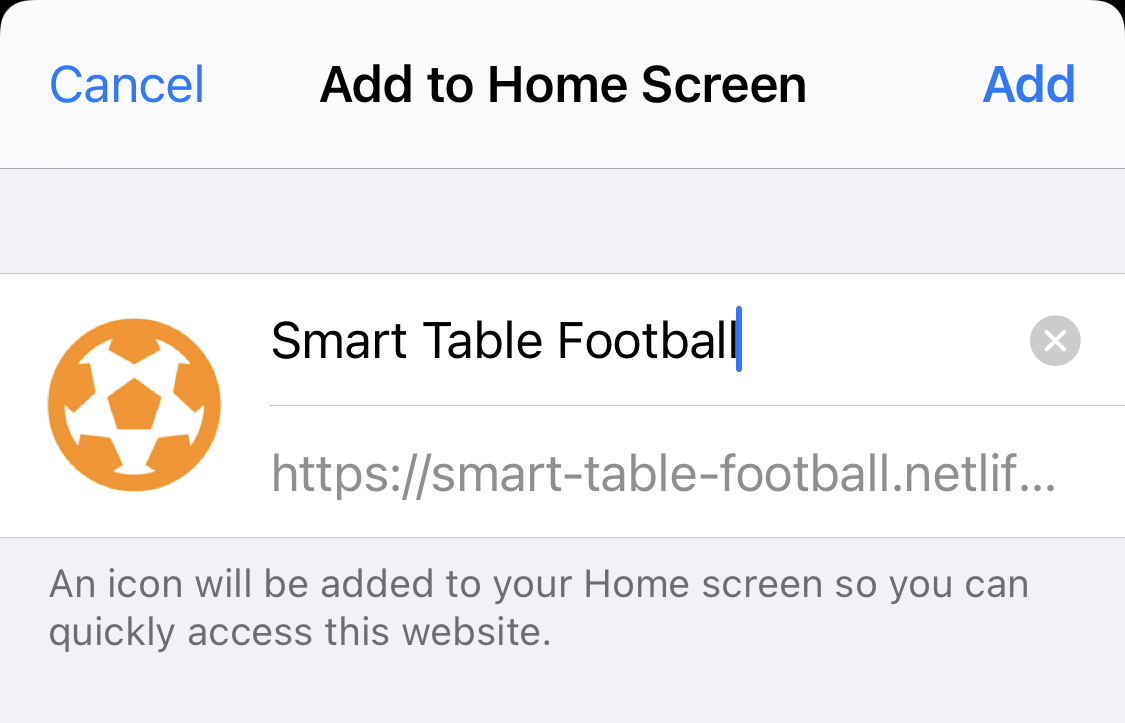
\includegraphics[width=0.5\textwidth]{images/player/PWA_install.jpg}
    \caption{Instalacja aplikacji PWA w systemie IOS}
    \label{fig:mobile}
\end{figure}

\section{Material UI}
Kolejną biblioteką JavaScript'ową zastosowaną w projekcie jest Material-UI. Jest to zbiór komponentów reactowych, rozwiajny przez firmę Google, opartych o zdefinowany i wysoco ceniony przez programistów zbiór zasad designu Material Design. Biblioteka ta pozwala na budowanie aplikacji z gotowych komponentów z możlwiością ich dostosywania i utrzymywania jednolitego stylu w całej aplikacji. Dzięki charakterystycznym komponentom graficznym użytkownicy aplikacji są w stanie znacznie szybciej dokonywać pożądanych akcji przez znane i popularne dla nich elementy graficzne. Wszystkie komponenty zachowują dobre praktyki dostępności oraz zapewniają swoją responsywność na różnych urządzeniach.

\section{React Admin}
Pakiety 'admin' oraz 'player' wykorzystują u swej podstawy framework 'React Admin'. Jest to narzędzie rozwijane od 2016 roku oraz tworzene przez fransuskie studio. Narzędzie to wyróznia się od pozostałych, tym że jest framework'iem a nie biblioteką. Główną róznicą jest narzeucenie pewnej struktury budowy aplikacji przez narzędzie. Początkowo, użycie tej technologii miało znaleźć swoje zastsowanie w projekcie tylko przy budowie panelu administracyjnego. Uniwersalność i wahalarz możliwości jakie oferuje to narzędzie w efekcie końcowym pozwiliło również na budowę aplikacji końcowej dla graczy.

Głównymi funkcjonalnościami jakie oferuje react admin i zostały wkorzystane w projekcie to:

\begin{itemize}
    \item Gotowy szkielet aplikacji
    \item Zestaw komponentów zbudowanych przy użyciu biblioteki Material UI
    \item Adapter warstwy komunikacyjnej (prosta komunikacjia z serwerem, który wykorzystuje Feathers.js)
    \item Warstwa autentykacji i autoryzacji
    \item Internacjonalizacja (Zapewnienie treści w różnych językach)
    \item Wkorzystuje swój własny wbudowany mechanizm cachowania
\end{itemize}

Narzędzie te pozwala na pełną modyfikowalność całego szkieletu interfejsu graficznego. Pakiet 'admin' został zbudowany praktycznie bez wprowadzania żadanych modyfikacji co do wyglądu aplikacji. Pakiet 'player' natomiast wymorzystał pełną gamme możliwości rozbudowy aplikacji oraz funkcjonalności tego framework'u.

\section{Storybook}
Ostatnim narzędziem użytym w części projektu służącej budowie interfejsu graficznego jest Storybook. Jest to narzędzie to budowania komponentów graficznych w odizolowaniu od ich logiki. W praktyce oznacza to, że programista może przykładowo stworzyć przycisk, który będzie przyjmował jakieś właśności takie jak kształt, kolor czy wariant i będzie mógł przetestować ich różne formy wyświetlania w zależności od tych parametrów bez podawania logiki, która mówić co taki przycisk ma robić.

W systemie znajdują się dwa pakiety zakładające budowe interfejsów graficznych, które wykorzystują nieraz te same komponenty lub konfiguracje. W celu uniknięcie duplikacji kodu powstał pakiet 'ui-components', którego głównym założeniem jest budowa komponentów wykorzystywanych w obydwu tych pakietów z pomocą Storybooka. Jedną z funkcjonalności tego narzędzia jest również autogenerowanie, z którego pomocą został skonfigurowany pakiet 'ui-components'. 

\begin{figure}[h!]
    \centering
    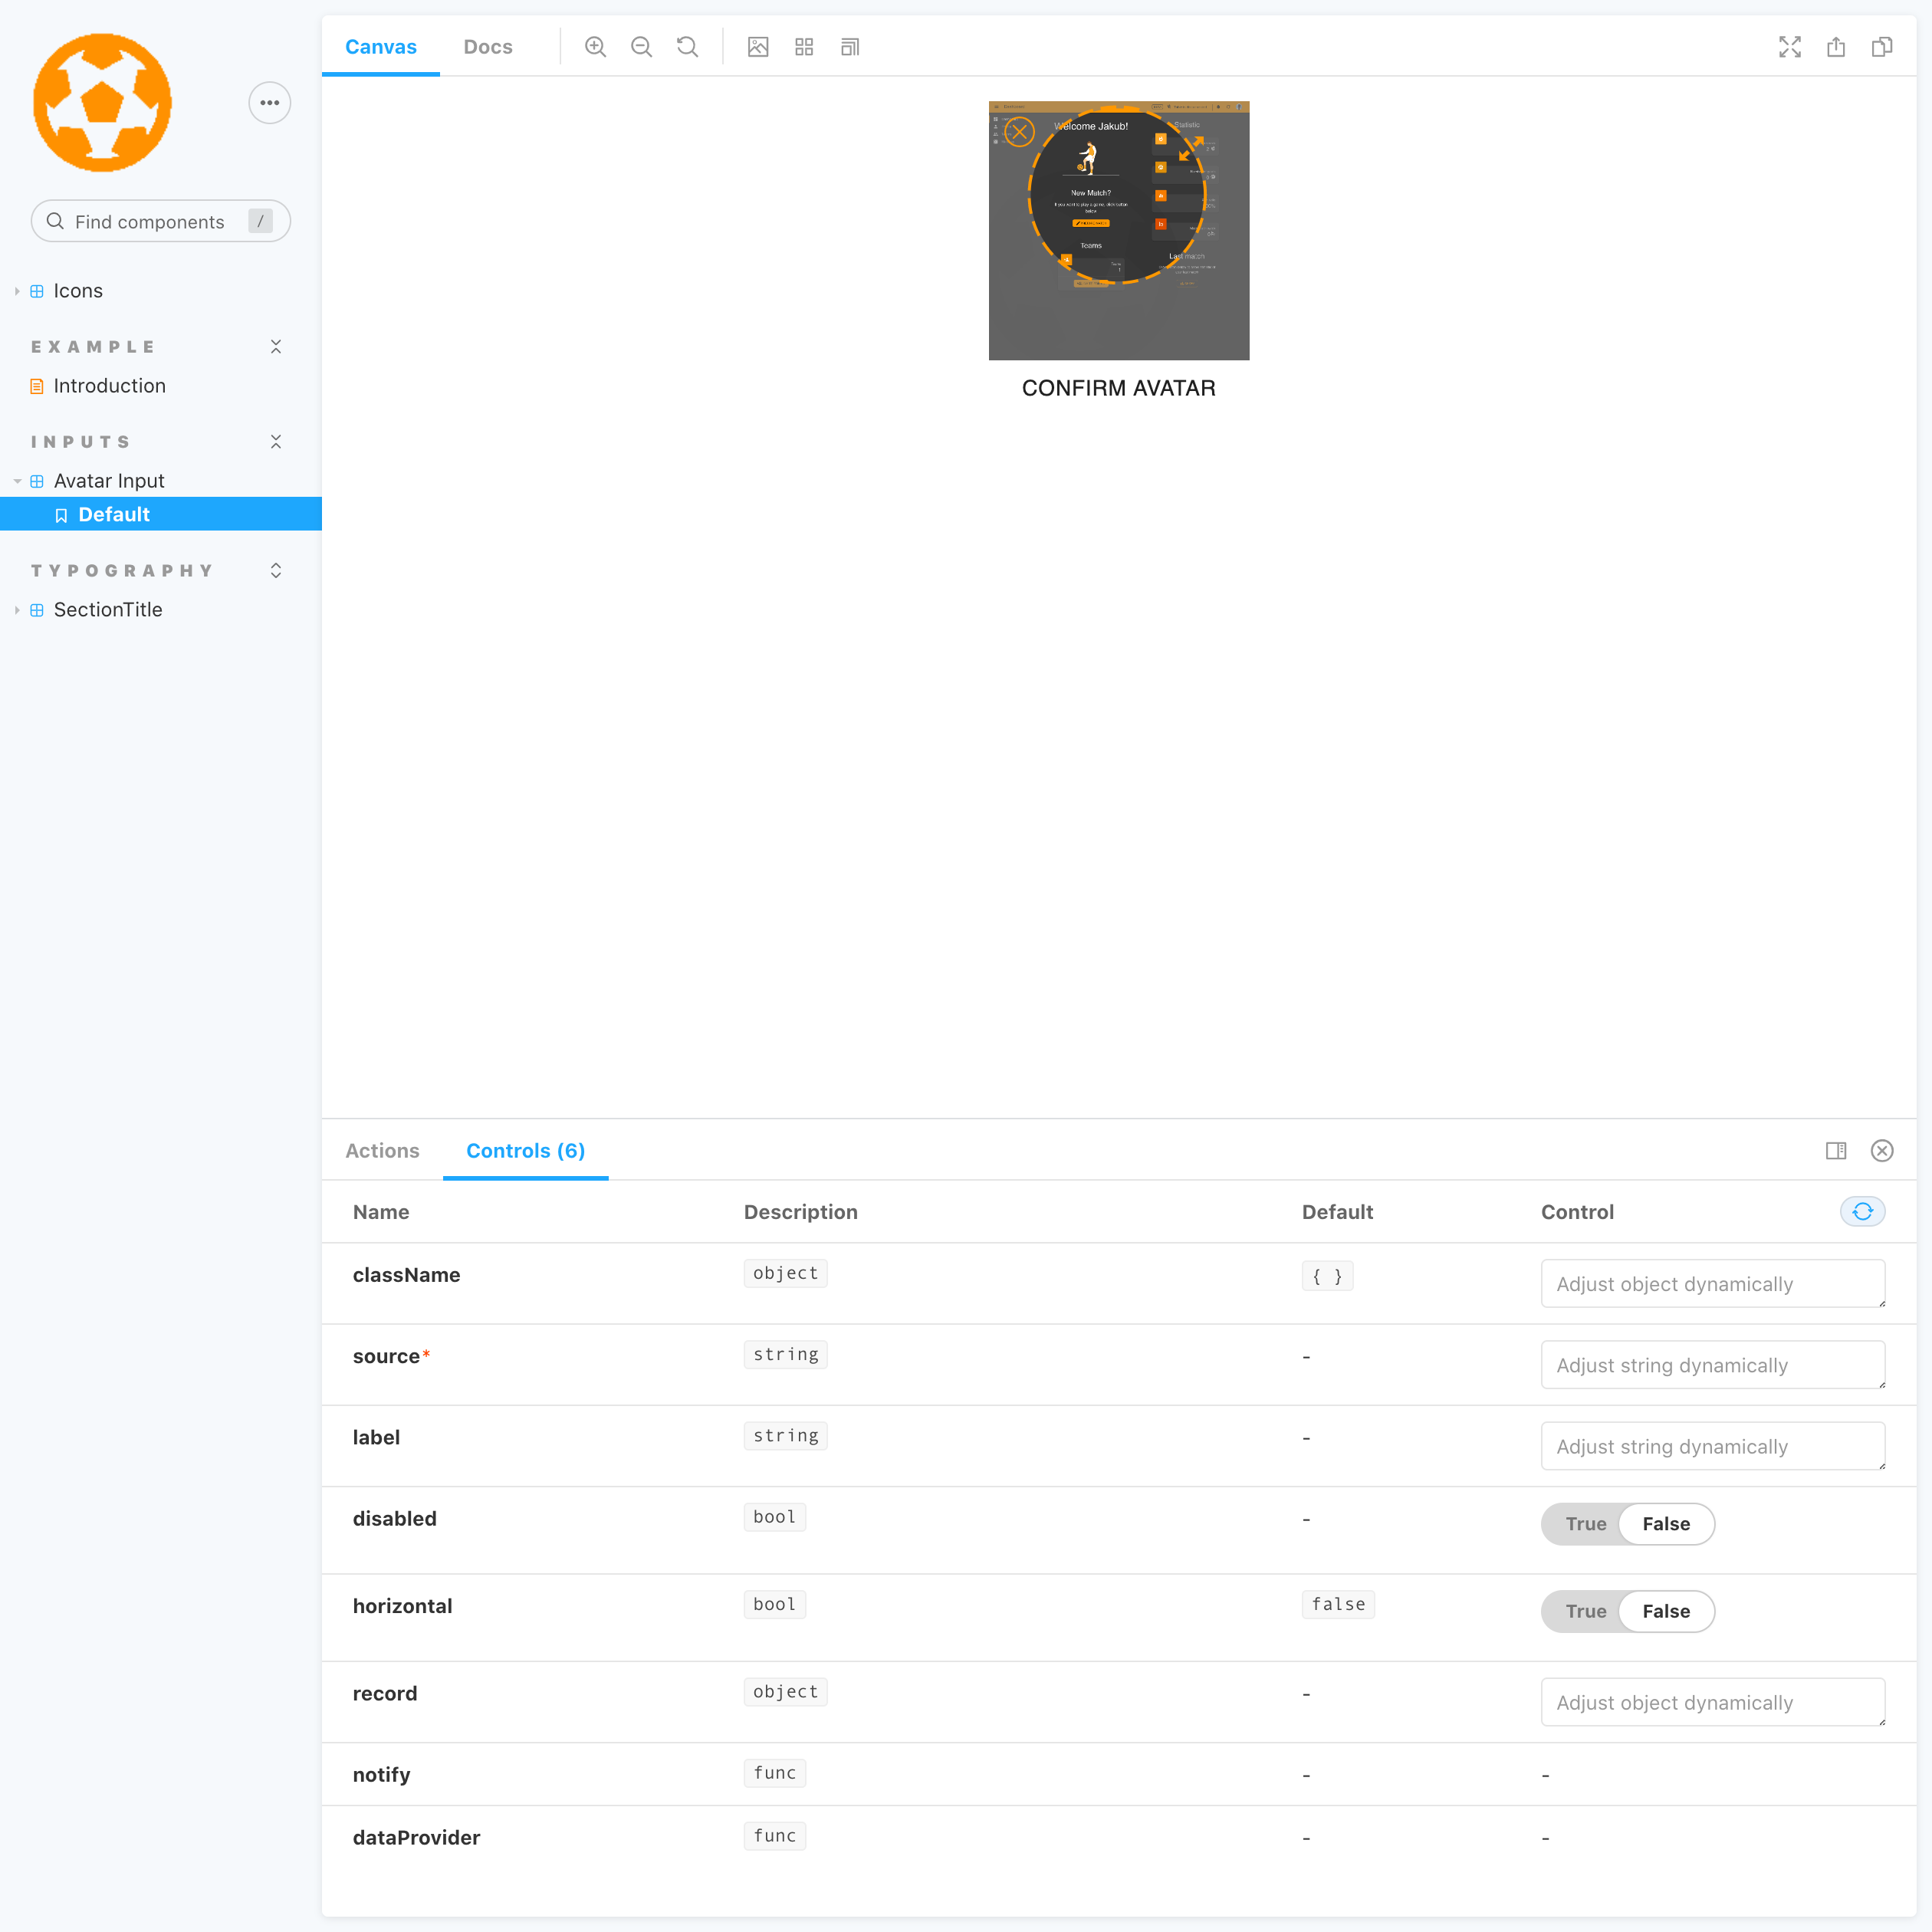
\includegraphics[width=0.5\textwidth]{images/ui-components/storybook.png}
    \caption{Działanie storybook}
    \label{fig:mobile}
\end{figure}
